\subsection{Teknologianalyse}
\label{sec:teknologianalyse}
Vi ser en tydelig mulighed for at assistere forbrugere med at træffe et valg når det kommer til (køb af vare på nettet | bestemmelse af optimale lysforhold i hjemmet | visualisering af et tilkøbt element i forbrugernes dagligdag/hjem). Dette vil sandsynligvis kunne løses ved hjælp af bedre købsvejledning eller værktøjer til at assistere forbrugeren i en købssituation hvor en prøve ikke kan stilles til rådighed eller at returnere varen er umuligt eller for omfattende en process.

% // redegørelse
Blot at vælge en lampe fra et katalog er problematisk hvis der ikke er billeder af lampen som 
\begin{enumerate}
    \item Fremviser lampen som møbel, rent visuelt, det fysiske design og 
    \item Viser hvordan lys kastes af lampen. En god løsning vil være at have en fysisk model placeret i en kontekst hvor man kan komme og se lampen og se lyset i sammenspil med anden indretning, sålledes som f.eks. Ikea gør.
\end{enumerate}

Man vil også kunne skabe billige prototyper af lamper vha. 3D printer tekniker. Disse ville eventuelt være mulige at tage med hjem for at teste hvordan en lampe passer ind i det rum den egentligt er købt til, men fordi plastik vejer mindre end metal, glas og andre tunge materialer som lamper kan være produceret af, kunne man forestille sig ophængs metoder der ikke nødvendiggør at bore huller i væge før man har set om lampen passer ind i rummet.

En tredje metode kunne være at konstruere en 3D model af lampen og køre en simulation af hvordan den kaster lys, dette koncept vil også kunne udvides til at en forbruger kan modellere deres eget hjem og placere lampen i den model, eller det kan anvendes af sælgere som et værktøj til at vejlede forbrugeren til at gøre det rigtige køb.

% Indledning over

\subsubsection{Teknologier til visualisering}
For at undersøge hvilke teknologier der kan anvendes til visualisering, er der i dette afsnit en række teknologier og metoder, som alle er relevante i forhold til at visualisere en lampe. Formålet med afsnittet er at få en forståelse af hvilke teknologier der allerede eksisterer inden for visualisering, og finde ud af hvilke metoder der er bedst i forhold til visualisering af lamper for forbrugere der handler via internettet.

\paragraph{Digitale billeder taget med et fysisk kamera}
Som beskrevet under afsnit \ref{sec:ehandel}, benytter e-butikker, sig ofte af billeder til at vise kunden deres varer over internettet. Et eksempel på dette er vist på figur \ref{fig:e_handel_lampebilleder}.

\begin{figure}[H]
    \centering
    \fbox{\rule{\textwidth}{5cm}}
    \caption{Billeder af lamper på e-butikken somelampstore.what}
    \label{fig:e_handel_lampebilleder}
\end{figure} 

I det viste tilfælde er visualiseringen skabt ved at tage billeder af lamperne med et kamera fra en bestemt vinkel, i en kontekst der typisk hænger sammen med lampetypen. 

Fordelen ved denne type af visualisering er at den giver et virkelighedstro billede af, hvordan lampen ser ud i den kontekst, som billedet er taget i. Ulempen er så at der ofte kun er et begrænset antal billeder til rådighed, hvilket kan medføre, at forbrugeren ikke kan se lampen fra alle vinkler og på den måde ikke kan visualisere lampen for sig. Derudover kan det være svært at se hvordan lyset udbreder sig fra lampen, da dette til dels afhænger af hvilken vinkel man ser lampen fra. 

Herudfra kan man kortfattet sige at visualisering af lamper gennem billeder taget med et fysisk kamera, giver et realistisk billede af lampen, men kun i den kontekst og vinkel billedet er taget i. 

\paragraph{3D print}
En teknologi som sælgeren vil kunne være i stand til at bruge er 3D printere. De fleste 3D printere kan typisk benytte to slags plastik: Acrylnitrol Butadien Styren (ABS) \cite{hvordan_3Dprinter} og Poly Lactic Acid (PLA) \cite{hvordan_3Dprinter}, plasten kommer som en lang tråd på en rulle, som bliver sat på siden af printeren. Plasttråden bliver herefter ført gennem et rør ned til 3D printerens hoved, lige før plasten kommer ud af hovedet bliver det varmet op til knap 200 grader \cite{hvordan_3Dprinter}. Den flydende plastik bliver nu lagt i tynde lag typisk op 0.1mm størrelse, derfor størkner plasten hurtigt og smelter sig sammen med det underliggende lag, det at printe et lag af gangen er en additiv produktionsmetode \cite{additiv_produktion}. 
\begin{figure}[H]
   \centering
   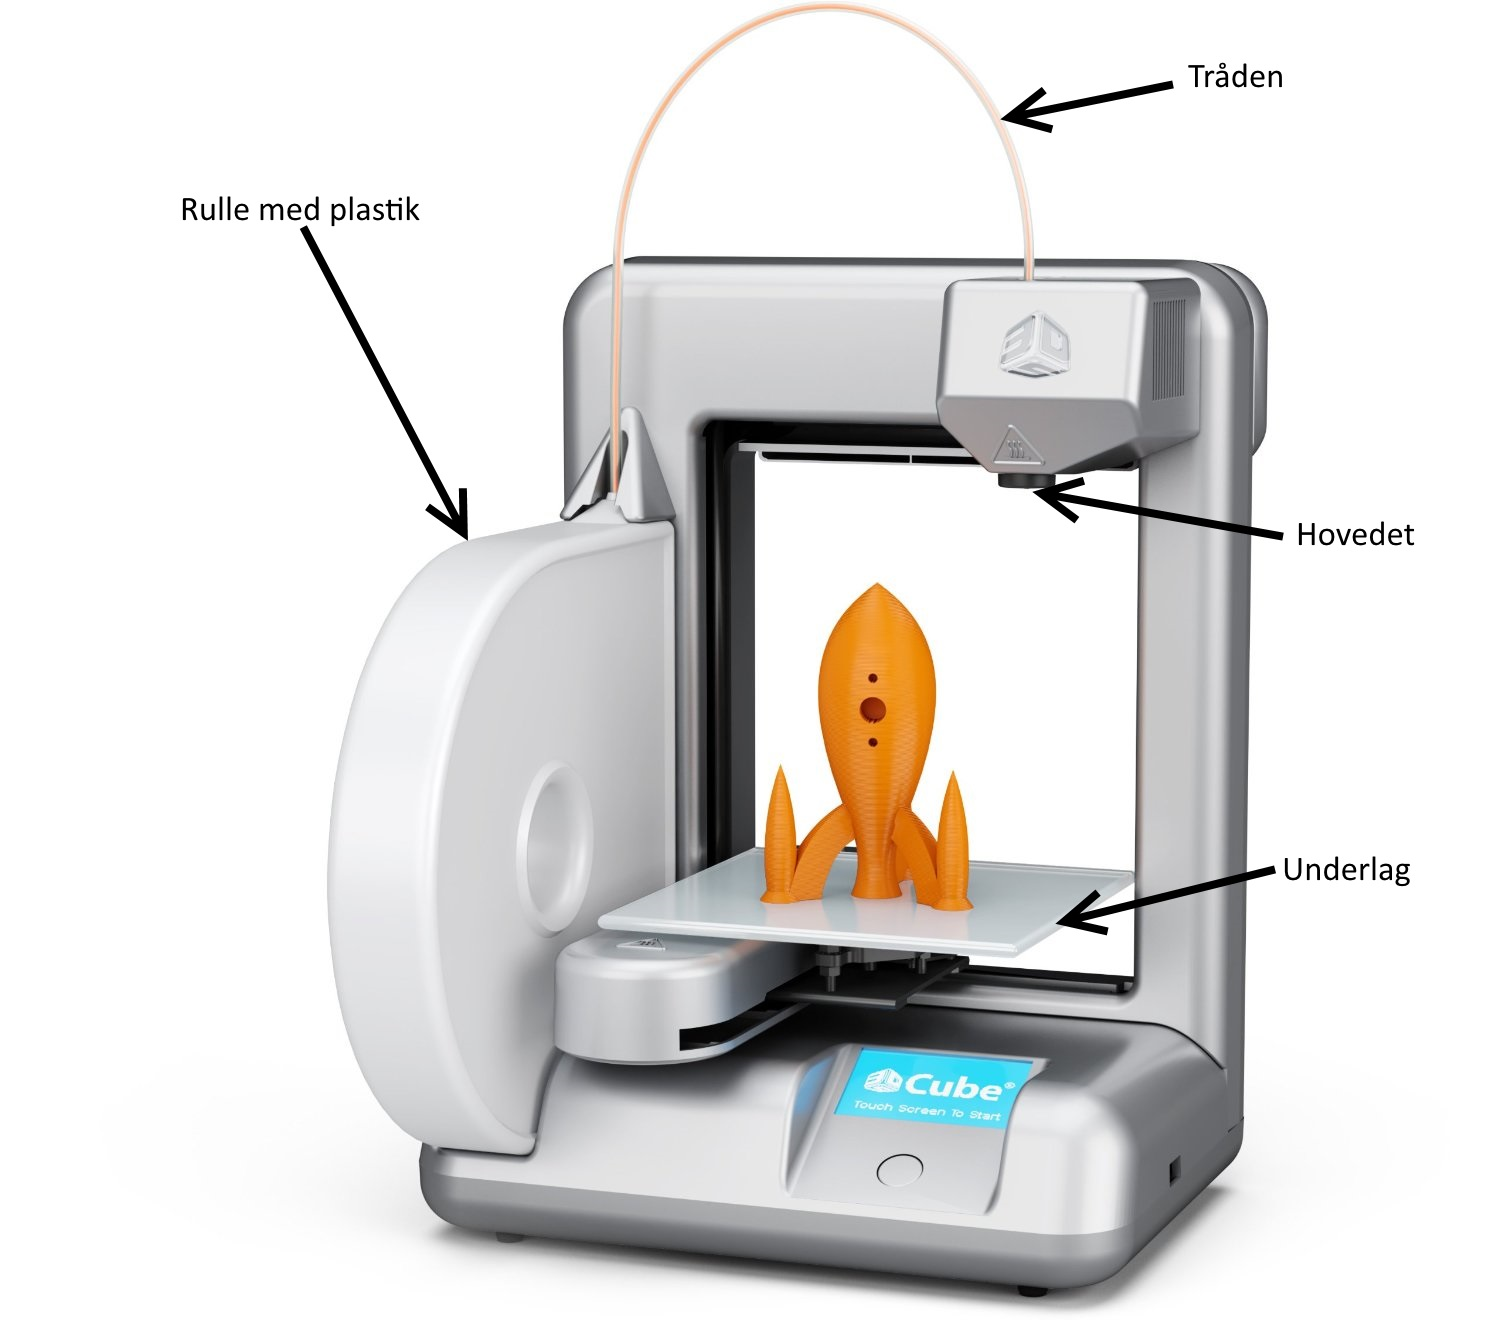
\includegraphics[width=10cm]{3D_printer_pil}
   \caption{Billede af 3D printer med pile til vigtige komponenter \cite{3D_printer_amazon}.}
\end{figure}
Sælgeren vil kunne bruge denne teknologi til at lave en demostrations vare som forbrugeren kunne tage med hjem, men da vi fokuserer på sælgere inden for e-handel vil dette ikke være en mulighed da e-handel som sagt ikke er en fysisk butik. I stedet kan sælgeren give forbrugeren en fil, så forbrugeren selv vil være i stand til at lave en 3D print af en bestemt lampe, dette vil dog kræve at forbrugeren har en 3D printer og masser af tid da store objekter generelt vil tage lang tid at lave, alt efter hurtigheden af printeren kan der går alt fra få minutter for en lille genstand til flere dage for en stor genstand \cite{hvordan_3Dprinter}. Derudover er 3D printere stadig en så ny teknologi at et 3D print nemt kan gå galt hvis maskinen ikke er kallibreret korrekt eller printeren er af lavere kvalitet, det er altså sjældent blot en \textit{one click print} løsning. Disse 3D printere varierer rigtigt meget i pris og funktionalitet, dog koster nogle af de gode 3D printer over titusinde kroner \cite{3D_printer}. 

Dette vil dog ikke være en fuldstændig løsning da forbrugeren stadig vil skulle hænge lampen op for at se lysets udbredelse. Desuden vil det være en dårlig ide for sælgere at forvente at deres kunder har en 3D printer derhjemme og det kan heller ikke forventes at forbrugerne investerer så mange penge på noget som de måske kun kommer til at bruge til at lave en lampe. Et andet problem er at sælgeren også kommer i et dilemma, da sælgeren skal bestemme om man kan få disse tegninger inden man har købt lampen eller om forbrugeren skal betale en form for depositum.

\paragraph{Computergrafik}
% Kilder:
% Rastarizering og lidt gennerelt http://people.csail.mit.edu/fredo/Depiction/1_Introduction/reviewGraphics.pdf
% Fotorealistisk 3D animation https://youtu.be/HjHiC0mt4Ts
Ved hjælp af mattematiske modeller og vektorbaserede beskrivelser af objekter kan computere bruges til at efterligne lys interaktion med simulerede fysiske objekter. Der eksistere en mængde forskællige metoder til dette formål, flere af hvilke kan bruges sammen med andre for at opnå et mere realistisk eller effektivt resultat. Der er ofte tale om en balance mellem hastighed og fotorealisme.
\begin{figure}[H]
    \centering
    %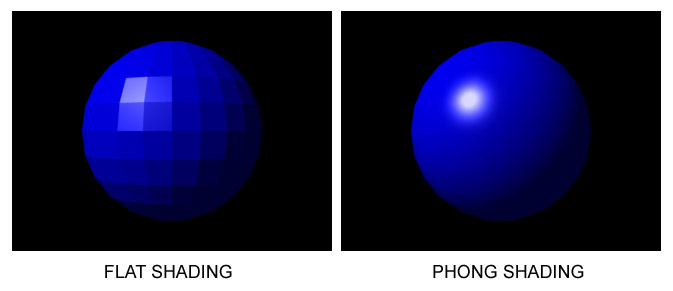
\includegraphics[width=\textwidth]{time_vs_quality}
    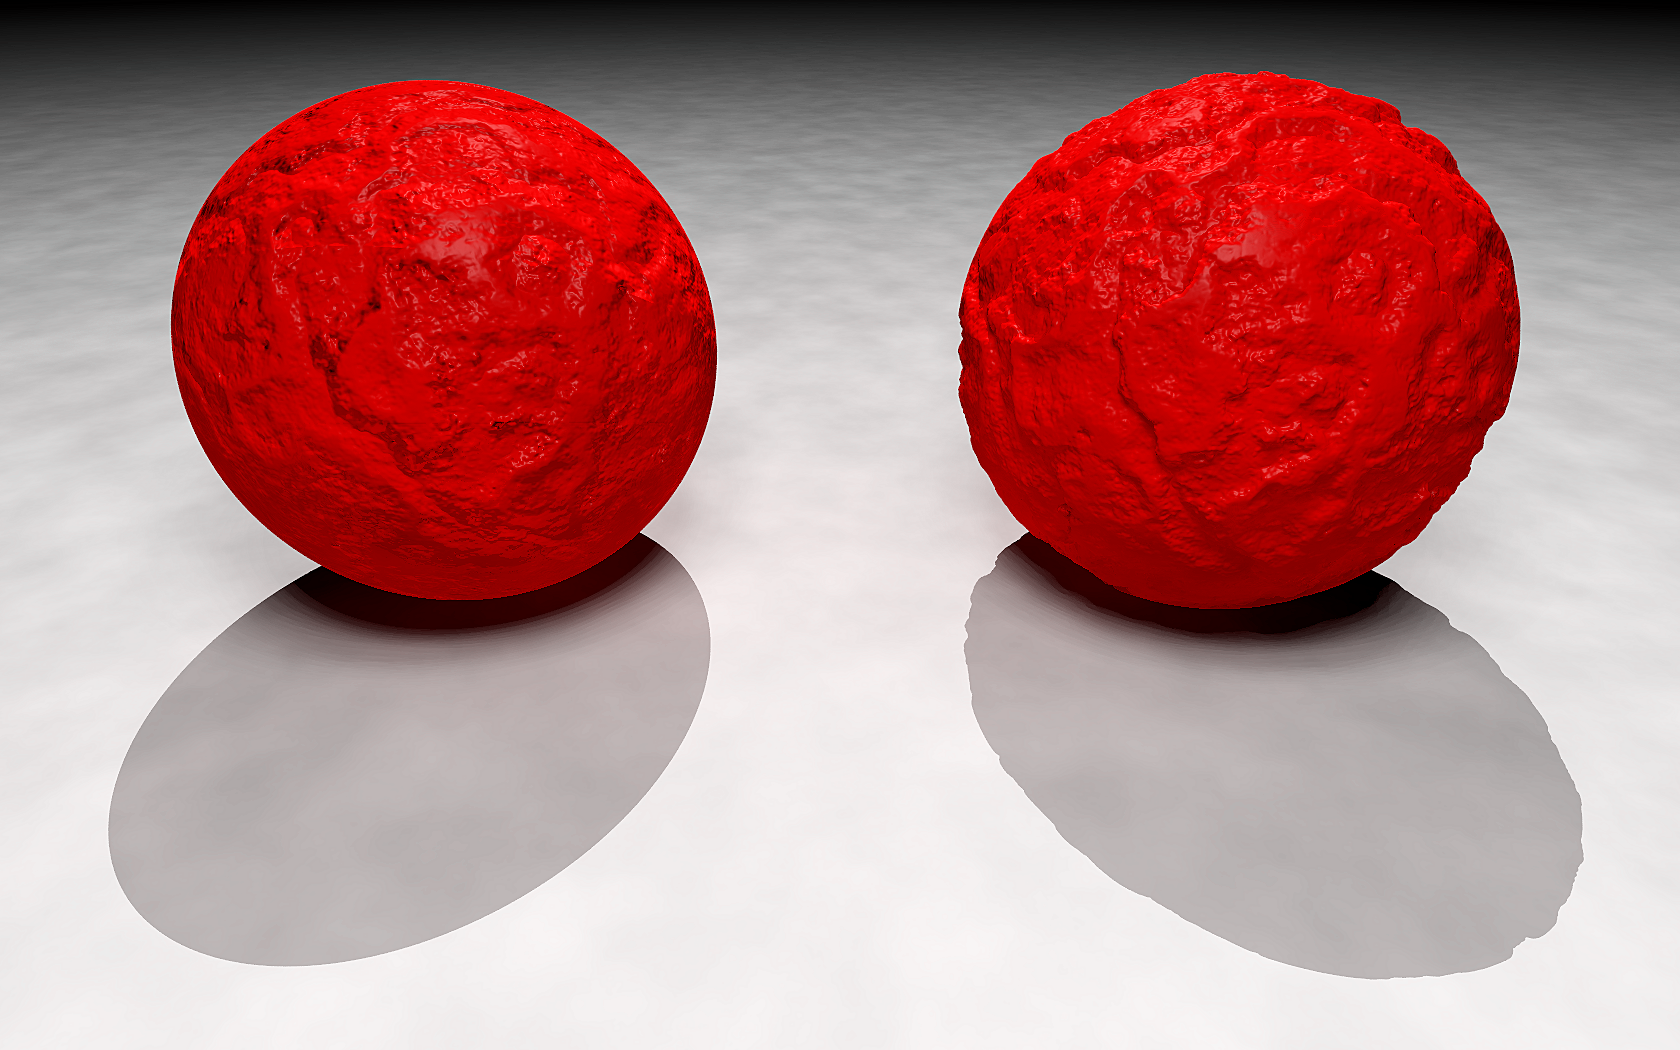
\includegraphics[width=12cm]{bumpmaps}
    \caption{Interpolation af flade-normaler kan få kantede figure til at få mere naturligt udseende.}
    \label{fig:tid_versus_kvalitet}
    % Demo der viser det samme http://math.hws.edu/graphicsbook/demos/c4/smooth-vs-flat.html
\end{figure}
\subparagraph{Rasterisering}
Den mest almindelige metode til at rendere miljøer med høj aktiv bruger interaktion er rasterisering. Rasterisering er også betegnelsen for at omdanne vector objekter til punkmatricer eller pixel-billeder (Se figur \ref{fig:pixelering}) Metoden virker ved at andvende linear transformationer på vektor objekter for at finde deres position på skærmen og derefter udfylde 2D polygonerne med farve, evt. baseret på forskællige lyskilder. Der kan dog simplificeres ved kun at andvende en ambient lys konstant. Rasterisering er også effektiv fordi grafikprocessore i computere er udviklet specifikt til at udføre matrix transformationer på store punktmængder.
\begin{figure}[H]
    \centering
    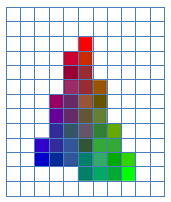
\includegraphics[width=6cm]{rastarization_aprox}
    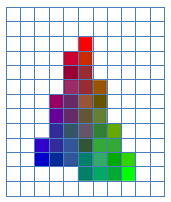
\includegraphics[width=6cm]{rastarization_aprox}
    \caption{Pixelering der fremkommer når vektor objekter rastariseres.}
    \label{fig:pixelering}
\end{figure}
\subparagraph{Ray tracing}
% Kilder
% https://www.cs.unc.edu/~rademach/xroads-RT/RTarticle.html
% 
Raytracing er en metode som med relative simple regler, forsøger at andvende en fysisk model af lys, hvor fotoner spredes fra en lyskilde og rammer forskællige objekter indtil nogle få rammer øjet eller kamerarets optik. 

Raytracing simplificere ved at reducere problemet til kun at simulere de stråler der rammer vores øje. Dette gøres ved såkaldt \textit{backward ray tracing} hvorved man følger en stråle fra øjet, igennem computerskærmen og ind i vektormodellen hvor man tjekker for kollisioner mellem strålen og objekter. Ved kollision med reflektiktive objekter som metaliske overflader og gennemsigtige objekter som glas, vil strålen nu dele sig og følge f.eks gennem glasset men også følge en reflektiv vinkel for at udregne farven som den gennemsigtige/reflektive overflade har. For hver kollision følger man også en stråle mod alle lyskilder for at teste om der er objekter i vejen, således at kollisionspunktet ligger i skygge, da dette tages i betragtning som farven udregnes. Ved kollision med et mat objekt eller efter en forudbestemt antal reflektioner/refraktioner stopper udregningen og propagere tilbage igen.
\subparagraph{Radiosity}
% Kilder
% http://web.cs.wpi.edu/~matt/courses/cs563/talks/radiosity.html 
% http://www.cs.bath.ac.uk/~pjw/NOTES/75-ACG/ch5-radiosity.pdf
Hvor Rasterisering og raytracing udregner en pixels farve baseret på hvad man kan se igennem en skærmflade, så er radiosity en metode som er uafhængig af hvor kameraret er placeret og er af samme grund en af de mest tidskrævende metoder. 

Radiosity er baseret på en fysisk forståelse af lys interaktion med flader og fungere ved at alle flader absorbere en del af lyset der rammer dem og reflektere(radiates) resten som så går videre til at gentage processen for andre flader i scenen. Ved radiosity er lyskilder selv geometriske flader, hvilket gør det nemt at beskrive elementer som lamper og el-pærer. Karakteristisk for denne metode er såkaldt \textit{color bleeding}, hvor farver fra forskællige objekter smitter af på hindanden.
\begin{figure}[H]
    \centering
    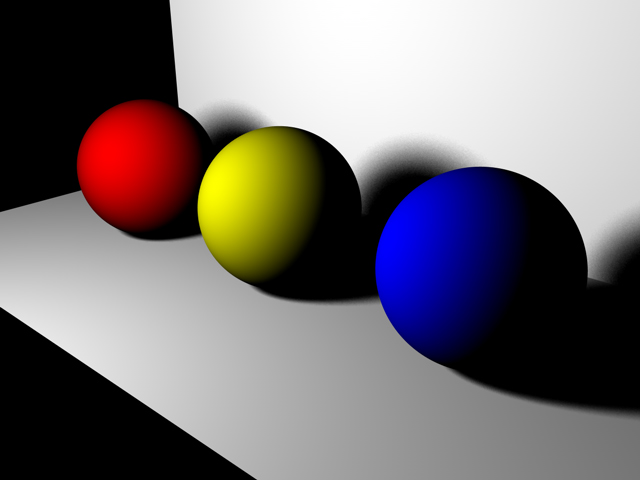
\includegraphics[width=6cm]{without_radiosity}
    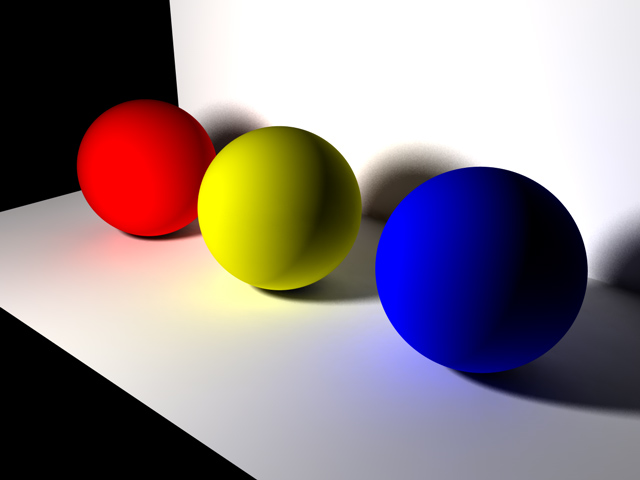
\includegraphics[width=6cm]{with_radiosity}
    \caption{\textit{Color bleeding} kan ses i billedet til højre.}
    \label{fig:colorbleeding}
\end{figure}

\paragraph{Opsummering}
Billeder af den fysiske lampe er en god og nem løsning på visualiseringsproblemet men computergrafik vil gøre det muligt for forbrugeren at se lampen fra flere vinkler hvor det måske er et større besvær for sælgeren at skaffe flere billeder af produktet istedet for blot at andvende en 3D model af lampen. Computergrafik giver også mulighed for nemt at se lampen i forskællige kontekster ved at udskifte miljøet som lampen bliver renderet i. 

Ideen om at printe en model af et lampe fra en e-butik for at se hvordan den rigtigt ser ud, er ikke en fornuftig løsning på nuværende tidspunkt, eftersom at 3D printere stadig er dyre og kan være svære at kallibrere korrekt. Computer grafik kan derimod nemt indlejres i en hjemmeside. Hvilken Computergrafisk teknik der er den korrekte er et case til case valg eftersom det helt afhænger af hvor meget fleksibilitet versus kvalitet der er nødvendigt. Radiosity giver, i de fleste tilfælde, den bedste kvalitet modsat rasterisering som til gengæld hurtigt kan tegne nye billeder og dermed tillader et stort nivau af bruger interaktion. Den gyldne middelvej kunne være raytracing som giver et lignende resultat, set i forhold til radiosity.